








\section{Features}
This section provides a deeper look into the user-facing features and technical aspects of the application.
\xxx{More user-focused documentation will be available in Chapter 6.}

\subsection{AuthX/Y}
The application includes user account functionality, supporting authentication and authorization.
Users can register, log in, and log out. Most pages and features are accessible only to logged-in users.

Passwords are hashed using \gls{sha256} encryption and must meet minimal requirements:
\begin{itemize}
\item At least 8 characters
\item At least one uppercase letter
\item At least one lowercase letter
\item At least one number
\end{itemize}

Login is managed via \gls{jwt} stored in \gls{local_storage}.
Tokens expire after one day, and a refresh token mechanism is not implemented, requiring users to re-login every 24 hours.

Tokens are currently sent in URL parameters for SignalR WebSocket connections.
This practice is not ideal and should be replaced in the future.
A possible solution involves a ticketing system where a logged-in client would request a ticket from the API.
This ticket would then authorize the WebSocket connection, avoiding token exposure in the URL. %\xxx{cit?}

\subsection{Pages}
Thanks to React, the graph view is one of many pages in the application. There are currently ten pages:
\begin{itemize}
\item \textbf{Homepage}: Displays a feed of recent thoughts and navigation buttons (Figure \ref{obr:afantazie_welcome_and_homepage})
\item \textbf{Welcome Page}: Similar to the homepage but tailored for unregistered users (Figure \ref{obr:afantazie_welcome_and_homepage})
\item \textbf{About Page}: Provides information about the project
\item \textbf{Chat Room}: A basic real-time chat
\item \textbf{Settings Page}: Contains user settings and a logout button
\item \textbf{Login and Registration Pages}
\item \textbf{Notifications Page}: Displays replies from other users
\item \textbf{Graph View}: Enables users to view thoughts
\item \textbf{Thought Creation Page}: Allows users to create new thoughts
\end{itemize}

\begin{figure}[p]
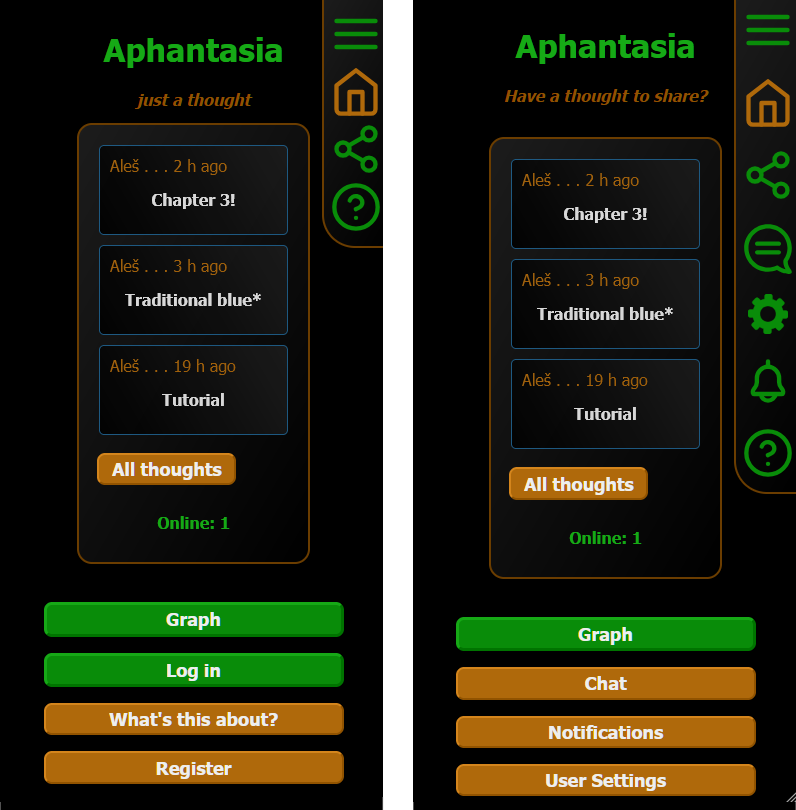
\includegraphics[width=130mm, keepaspectratio]{img/afantazie_welcome_and_home_page.png}
\caption{The Welcome page and homepage of Aphantasia}
\label{obr:afantazie_welcome_and_homepage}
\end{figure}

\subsection{Localization}
Initially, we developed a Czech version of the application and later added an English version.
For frontend \gls{localization}, we utilized two JSON files and a Localization object which returns 
either czech or english text based on \gls{vite} configuration.
This makes the application easily extensible to more languages.

Backend localization was also required, as the API returns localized authentication and validation messages.
To achieve this, we created a Localization project with classes implementing localization interfaces.
During boostrapping a specific localization is registered based on configuration. 
While this approach is somewhat cumbersome, it suffices for the limited localization needs of the backend.

\subsection{Custom Graph Rendering Engine}

The graph view is the primary feature of Aphantasia and the most complex part of the application.
Its basic features include:
\begin{itemize}
\item \textbf{Zooming and Panning}
\item \textbf{Dragging Thoughts}
\item \textbf{Floating Text Titles} (Figure \ref{obr:afantazie_floating_titles})
\item \textbf{Thought Highlighting} (On Figure \ref{obr:afantazie_mobile_graph_view} and \ref{obr:afantazie_floating_titles})
\end{itemize}

\begin{figure}[p]
    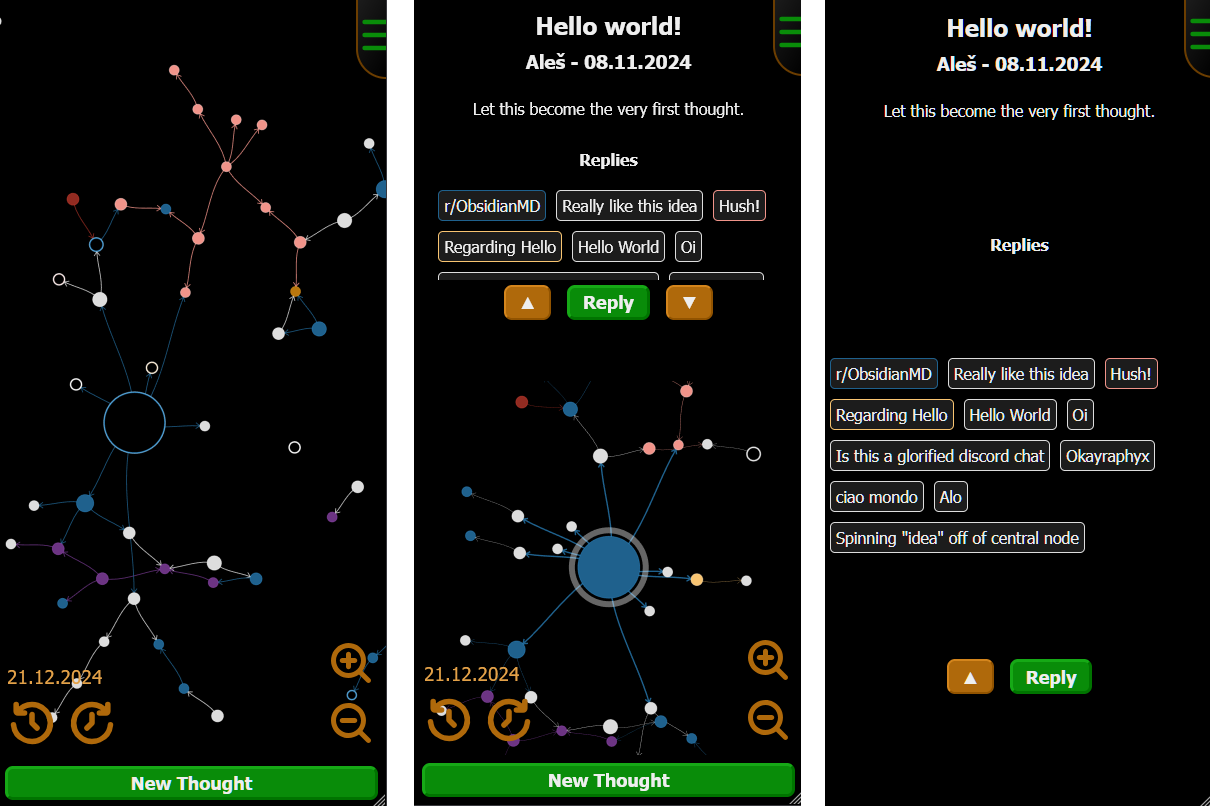
\includegraphics[width=130mm, keepaspectratio]{img/afantazie_mobile_graph_view.png}
    \caption{The graph view on mobile device - non-highlighted mode, half-screen preview and fullscreen preview respectively}
    \label{obr:afantazie_mobile_graph_view}
\end{figure}


\begin{figure}[p]
    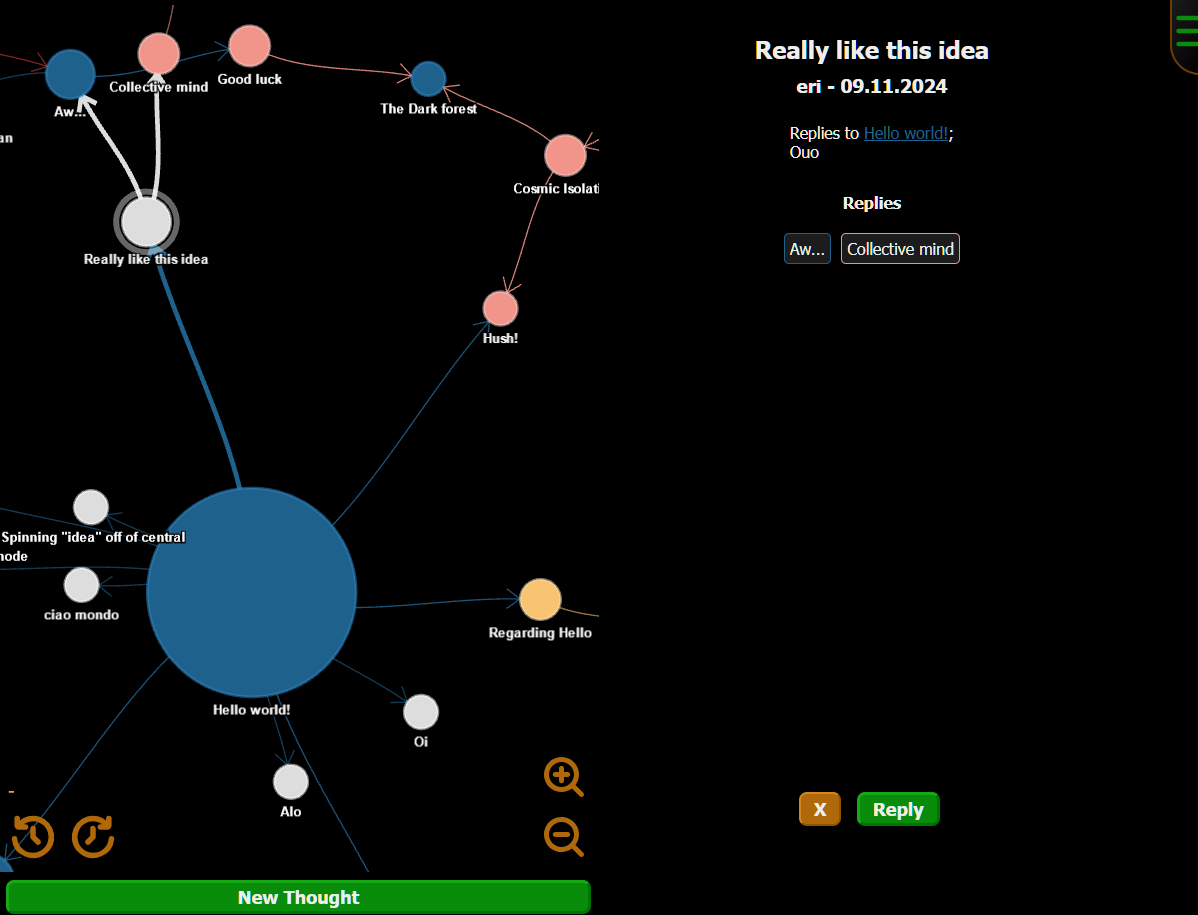
\includegraphics[width=130mm, keepaspectratio]{img/afantazie_floating_titles.png}
    \caption{Floating titles in the graph view on desktop}
    \label{obr:afantazie_floating_titles}
\end{figure}

% The graph view utilizes Pixi.js for rendering, \gls{zustand} for state management, and a custom \gls{FDL} implementation.
% move to implementation- todo

We began with pull and push forces and incrementally introduced a range of parameterizable settings to the computation.


\xxx{see documentation for the list of all available parameters.}

\begin{figure}[p]
    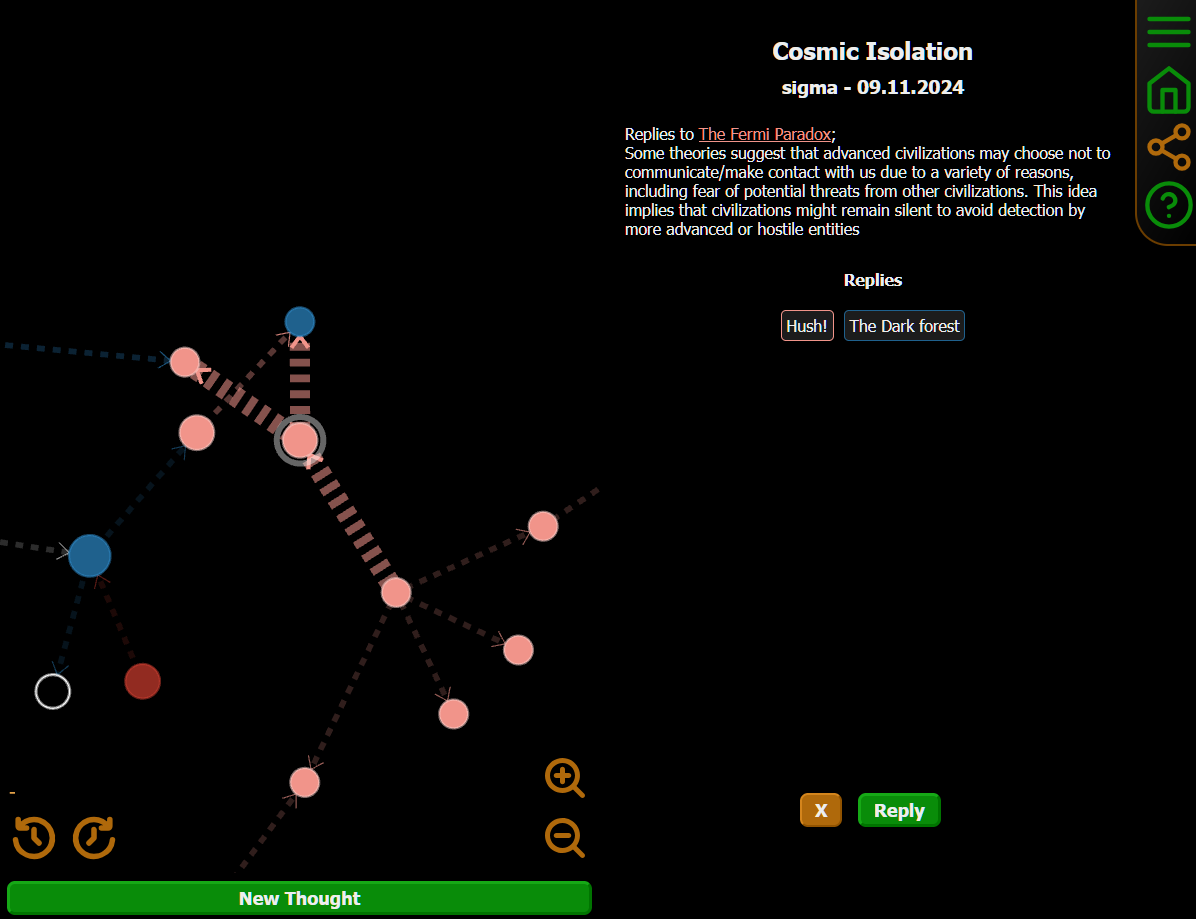
\includegraphics[width=130mm, keepaspectratio]{img/afantazie_animated_edges.png}
    \caption{Animated edges in the graph view}
    \label{obr:afantazie_animated_edges}
\end{figure}

\subsubsection*{On-screen thoughts limit}
The On-screen thoughts limit is a critical part of our big graph rendering solution.
The default value is 100, but users can adjust it in the settings.

The idea behind it is to always render at most this number of thoughts on screen.
And to view more user input is required - either by moving the time slider or by using the Graph walk feature, both of which we will talk about briefly.

The limit is demonstrated in Figure \ref{obr:afantazie_production_dataset_in_time_window} and \ref{obr:afantzazie_production_dataset_640_nodes} with the values set to 300 and 700 respectively.

\subsubsection*{Time Slider}
Combining the On-screen thoughts limit, dynamic loading, and two UI buttons resulted in a feature we call the Time slider.
It allows users to move a conceptual time window smoothly into the past or future by holding the corresponding button.
The resulting layout using time slider is demonstrated in Figure \ref{obr:afantazie_production_dataset_in_time_window}
with 641 thoughts on afantazie.cz viewed in three different time windows of length 300.

Above the time slider controls there is a label showing the current time window's position - the creation date of the newest thought on screen.
The label can be seen in bottom left in Figure \ref{obr:afantazie_mobile_graph_view}.

New thoughts appear either in their cached positions (see Layout caching section below) or in a circular pattern around the simulation container’s center.
When not yet cached the appearance of newer/older nodes creates a visually appealing effect as the thoughts gradually appear in what resembles a loading spinner.

\subsubsection*{Live Preview}
When the time slider moves beyond the last thought, the application enters live preview mode indicated by 'Now...' apearing in place of the time window's date in bottom left.
In this mode the client listens for new thoughts and adds them to the graph in real time.

While this feature enhances interactivity, it has only been tested with two users creating thoughts simultaneously.
Higher activity levels could potentially overwhelm the interface but until there is an active userbase this remains
a theoretical concern.

We implemented this feature using long polling, meaning that the client periodically sends
requests to the server to check for new thoughts. This approach is a bit wasteful, especially considering that we already have active
signalR connection to use across the entire appliction.
In the future we will replace long polling with the active signalR connection.

\subsubsection*{Graph Exploration}
The neighborhood API endpoint powers Graph walk demonstrated in Figure \ref{obr:afantazie_mobile_graph_view}.
After clicking on a node, link or reply the client loads the neighborhood of the newly highlighted thought, enabling interactive exploration.

In the example as well as many other screenshots provided in this work, some thoughts appear hollowed out.
This effect triggers when thought's direct neighbors (links or replies) are not currently rendered on screen
signalling that there is more to explore behind it.
When the neighbors of a node are all visible, the node is filled with its author's color.

Currently graph walk doesn't respect the on-screen thoughts limit and loads all neighbors of the highlighted thought up to given depth. This didn't pose a problem with the datasets we used but could be a significant issue with highly connected datasets.

\subsubsection*{Thoughts Layout Caching}
The browser’s local storage caches the thoughts layout after a period of inactivity.
The length of this period is parametrizable by number of frames,
with the current value set to 1000 frames which corresponds to around 30 seconds of inactivity on most devices.
When a thought leaves the screen and later reappears, it retains its previous position.
This feature facilitates graph stability during time sliding and between sessions and removes the need for the graph to re-stabilize again and again.

Paired with the Time slider this approach produced an unexpected emergent behavior. As the \gls{production} dataset grew beyond 500 thoughts (five times the default on-screen limit), it remained possible to create a stabilized graph across the entire dataset.
Moving the time slider across such stabilized layout is a uniquely satisfying experience, which we believe sets Aphantasia apart.
To some extent, this feature is visible in Figure \ref{obr:afantazie_production_dataset_in_time_window} but it is best experienced in the live application.

The cache currently has no size limit and is not cleared automatically, which could be a potential issue with big datasets and longer graph view sessions.
Logged in users can however delete cached positions in settings to force the graph to re-stabilize.

\begin{figure}[p]
    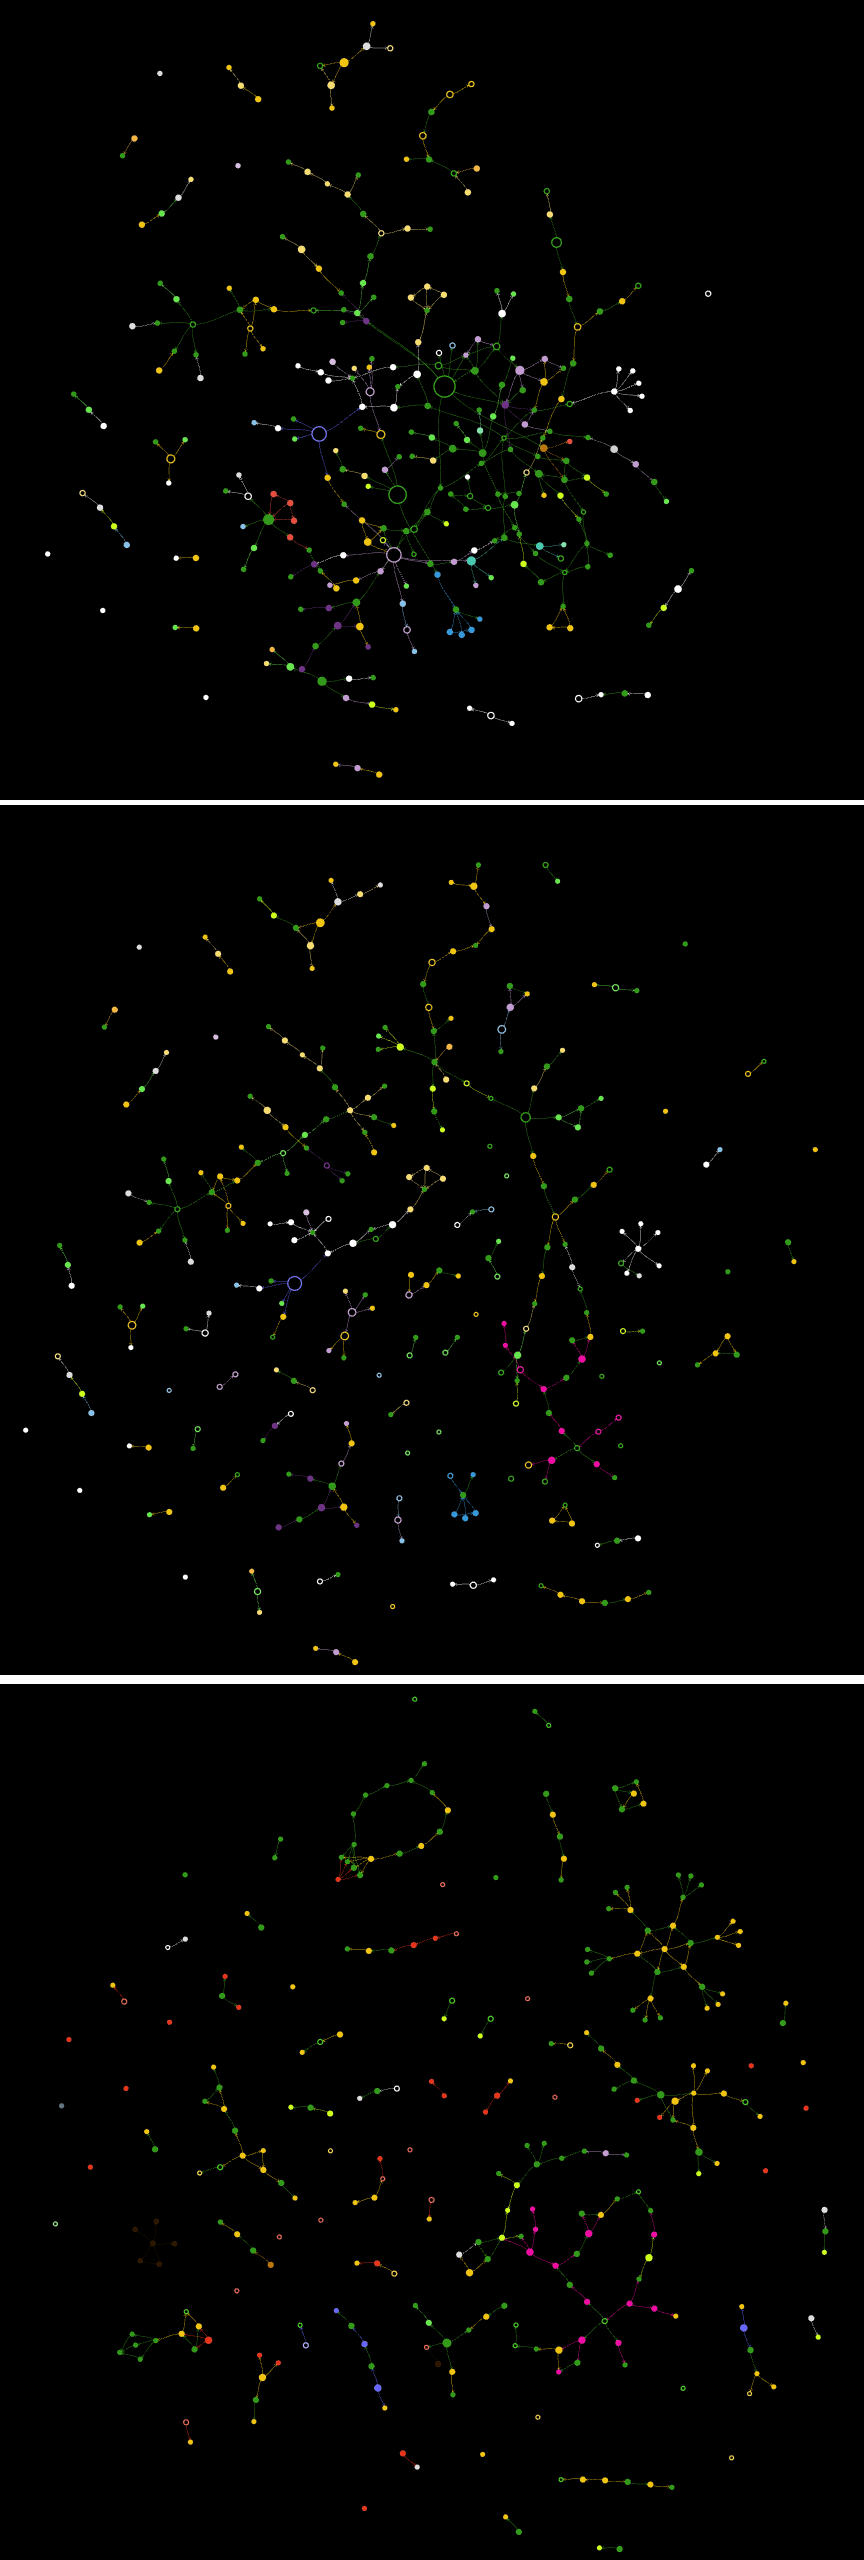
\includegraphics[height=200mm, keepaspectratio]{img/afantazie_production_dataset_in_time_window.png}
    \caption{Aphantasia with the czech production dataset in stabilized temporal layout (641 nodes in three time windows of length 300)}
    \label{obr:afantazie_production_dataset_in_time_window}
\end{figure}

\begin{figure}[p]
    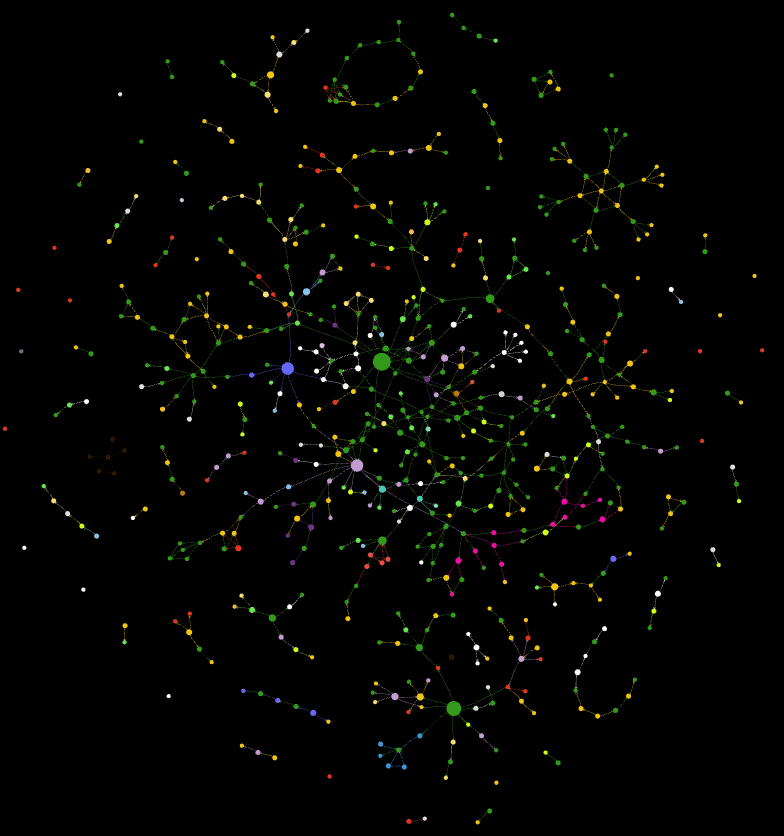
\includegraphics[width=130mm, keepaspectratio]{img/afantzazie_production_dataset_641_nodes.png}
    \caption{The entire dataset of afantazie.cz (641 nodes) in a single time window}
    \label{obr:afantzazie_production_dataset_640_nodes}
\end{figure}



